\documentclass{article}


%% We should use this latex document to store all the figures and
%% tables, and then do "make" to generate the floats.pdf which we will
%% send along with the main manuscript text.
\usepackage[a4paper,margin=2cm]{geometry}
\usepackage{graphicx}
\usepackage{mathpazo}
\usepackage{tabularx}
\usepackage[table]{xcolor} 

\begin{document}
\pagestyle{empty}


%% One float per page:
%% http://tex.stackexchange.com/questions/22191/forcing-a-figure-strictly-on-a-separate-page
\makeatletter
\@fpsep\textheight
\makeatother

\begin{figure}
  \centering
  \fbox{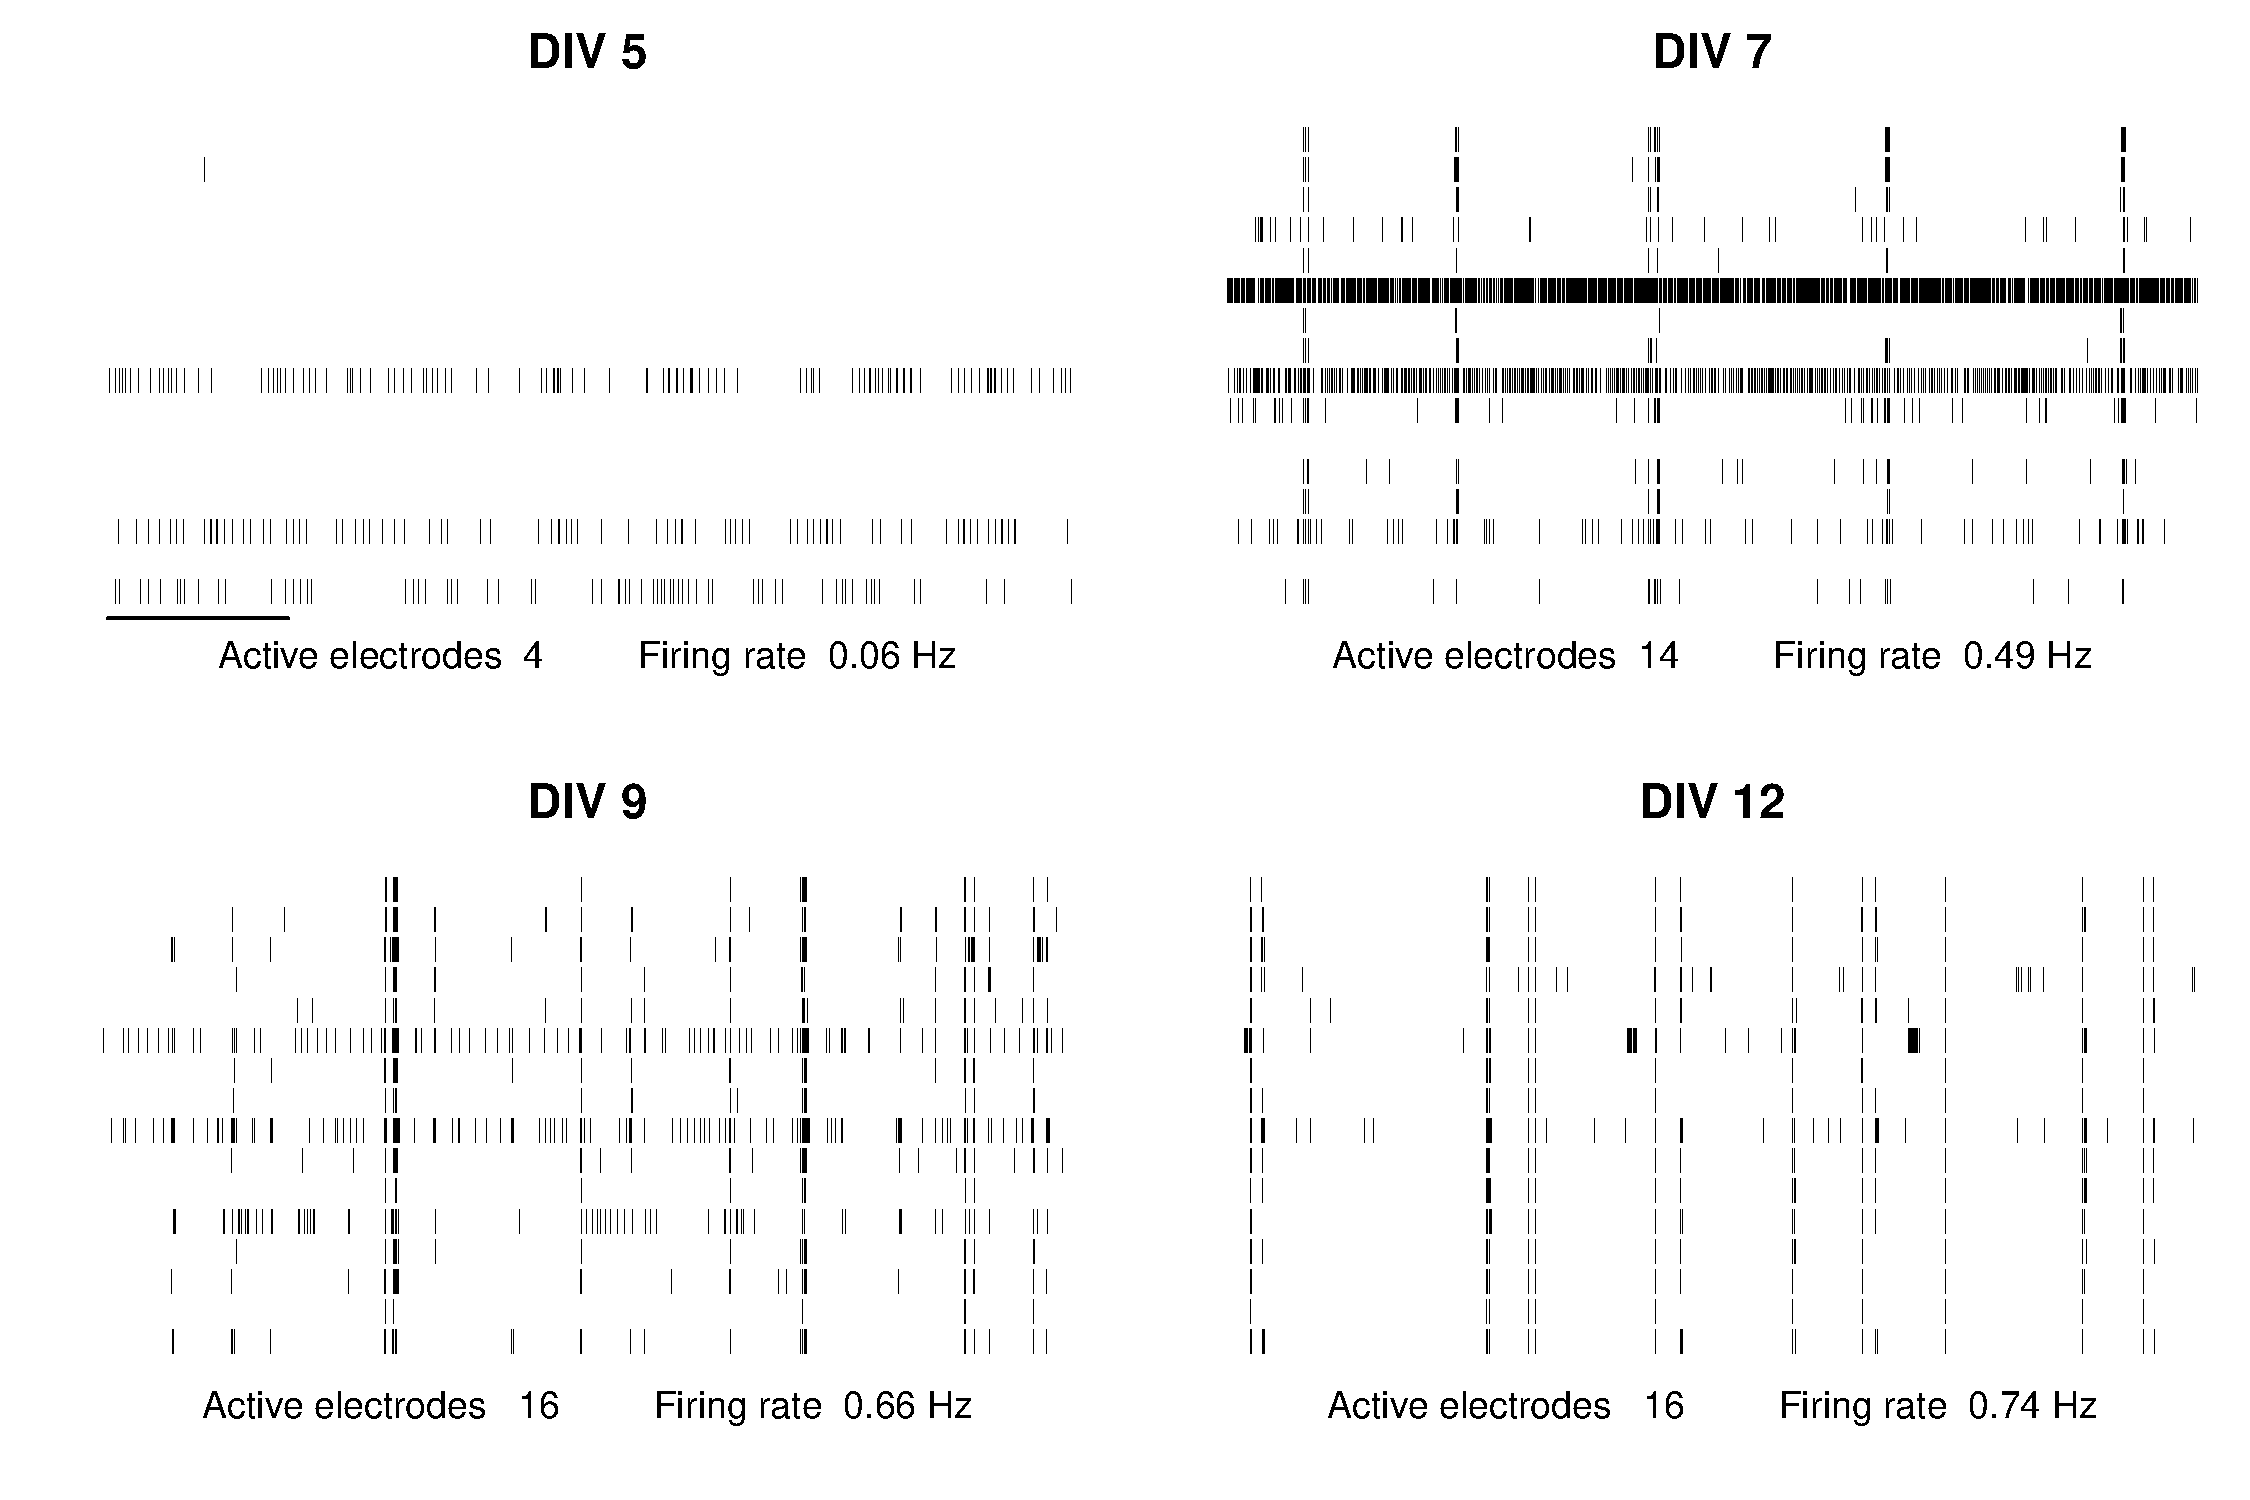
\includegraphics[width=170mm]{rasters.pdf}}
  \caption{Example raster plot from one well over the four DIV
studied. Each row represents the spike train from one electrode. The
scale bar for all raster plots is 60s.}
\end{figure}

\begin{figure}
  \centering
  \fbox{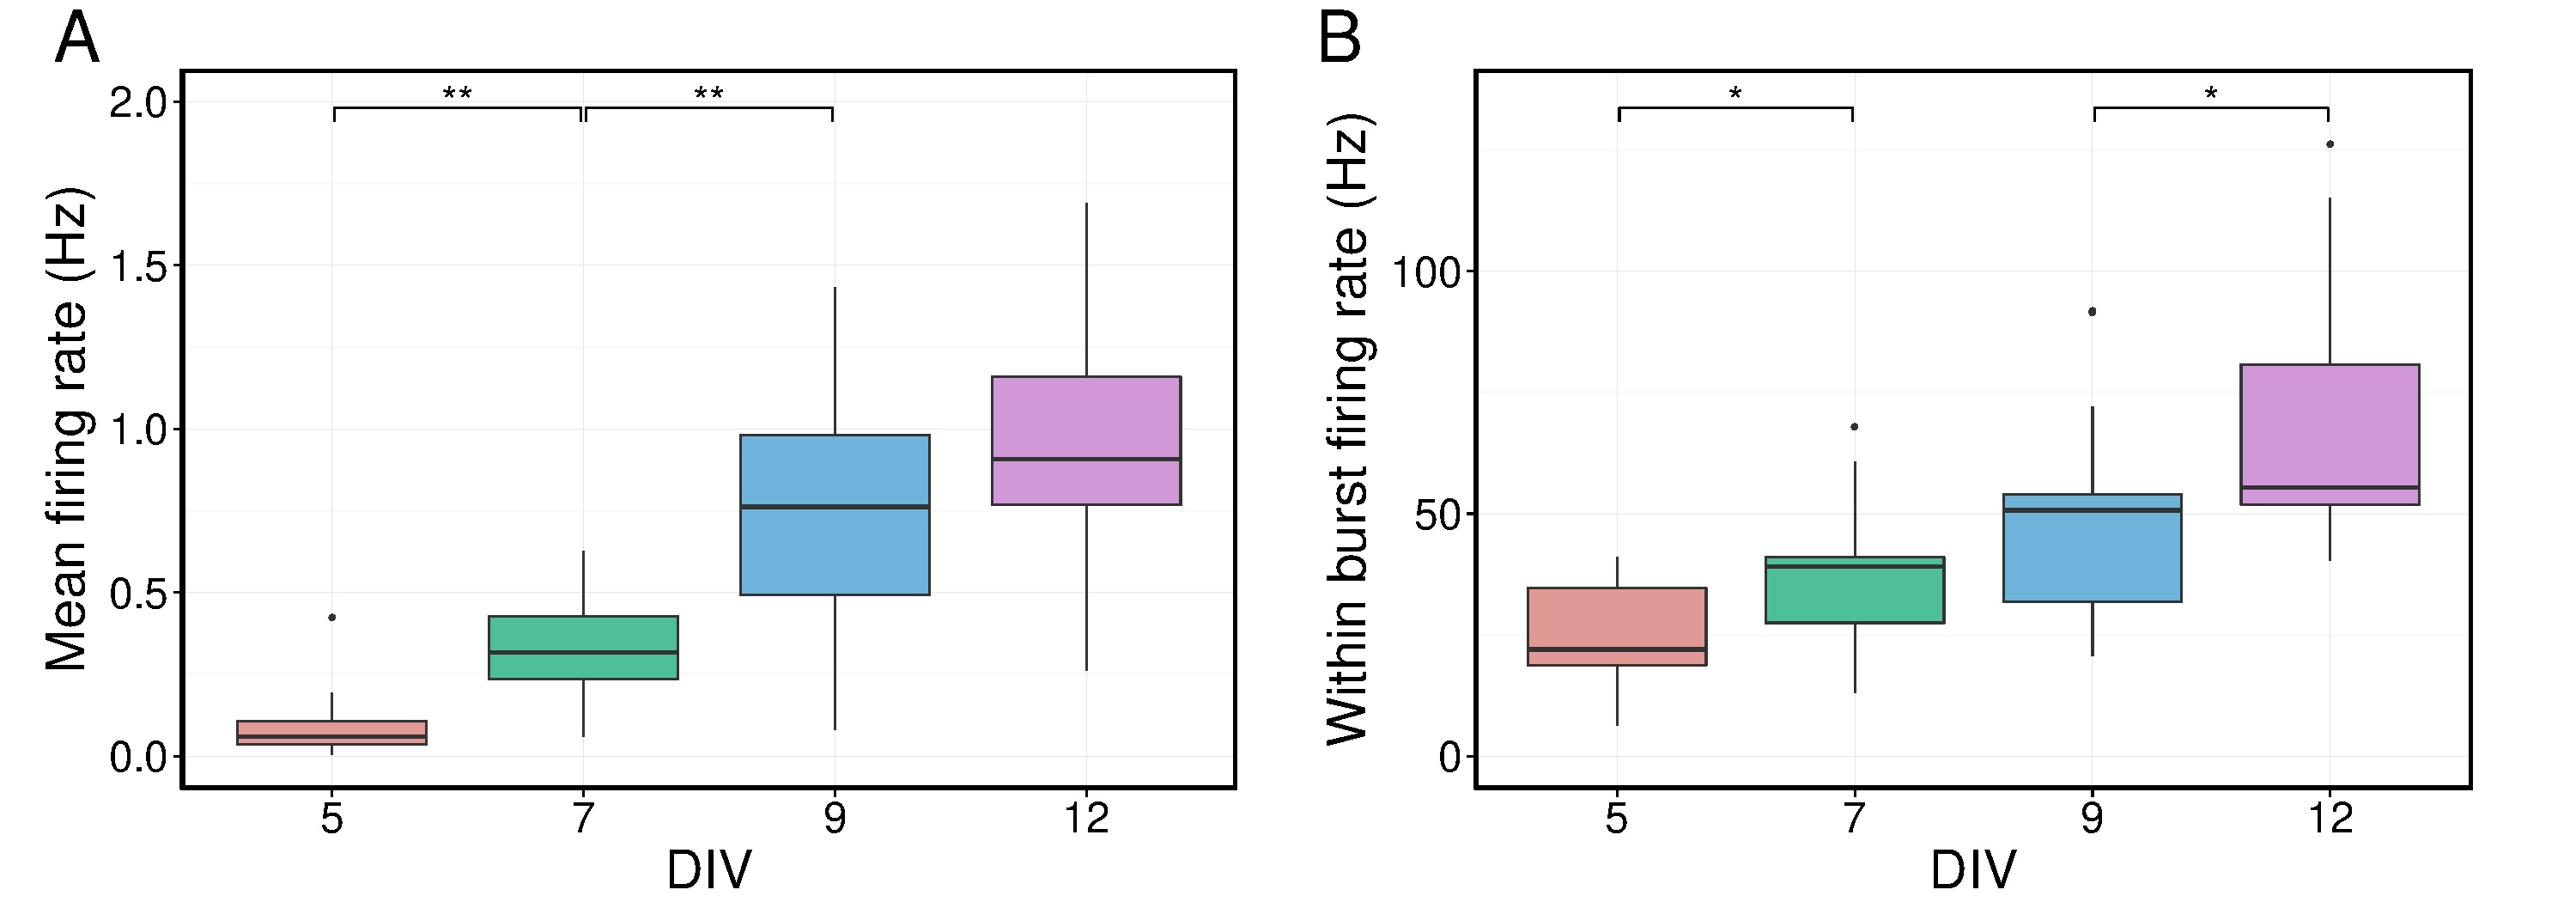
\includegraphics[width=170mm]{firingrate.pdf}}
  \caption{A Firing rate, and B within burst firing rate.}
\end{figure}

\begin{figure}
  \centering
  \fbox{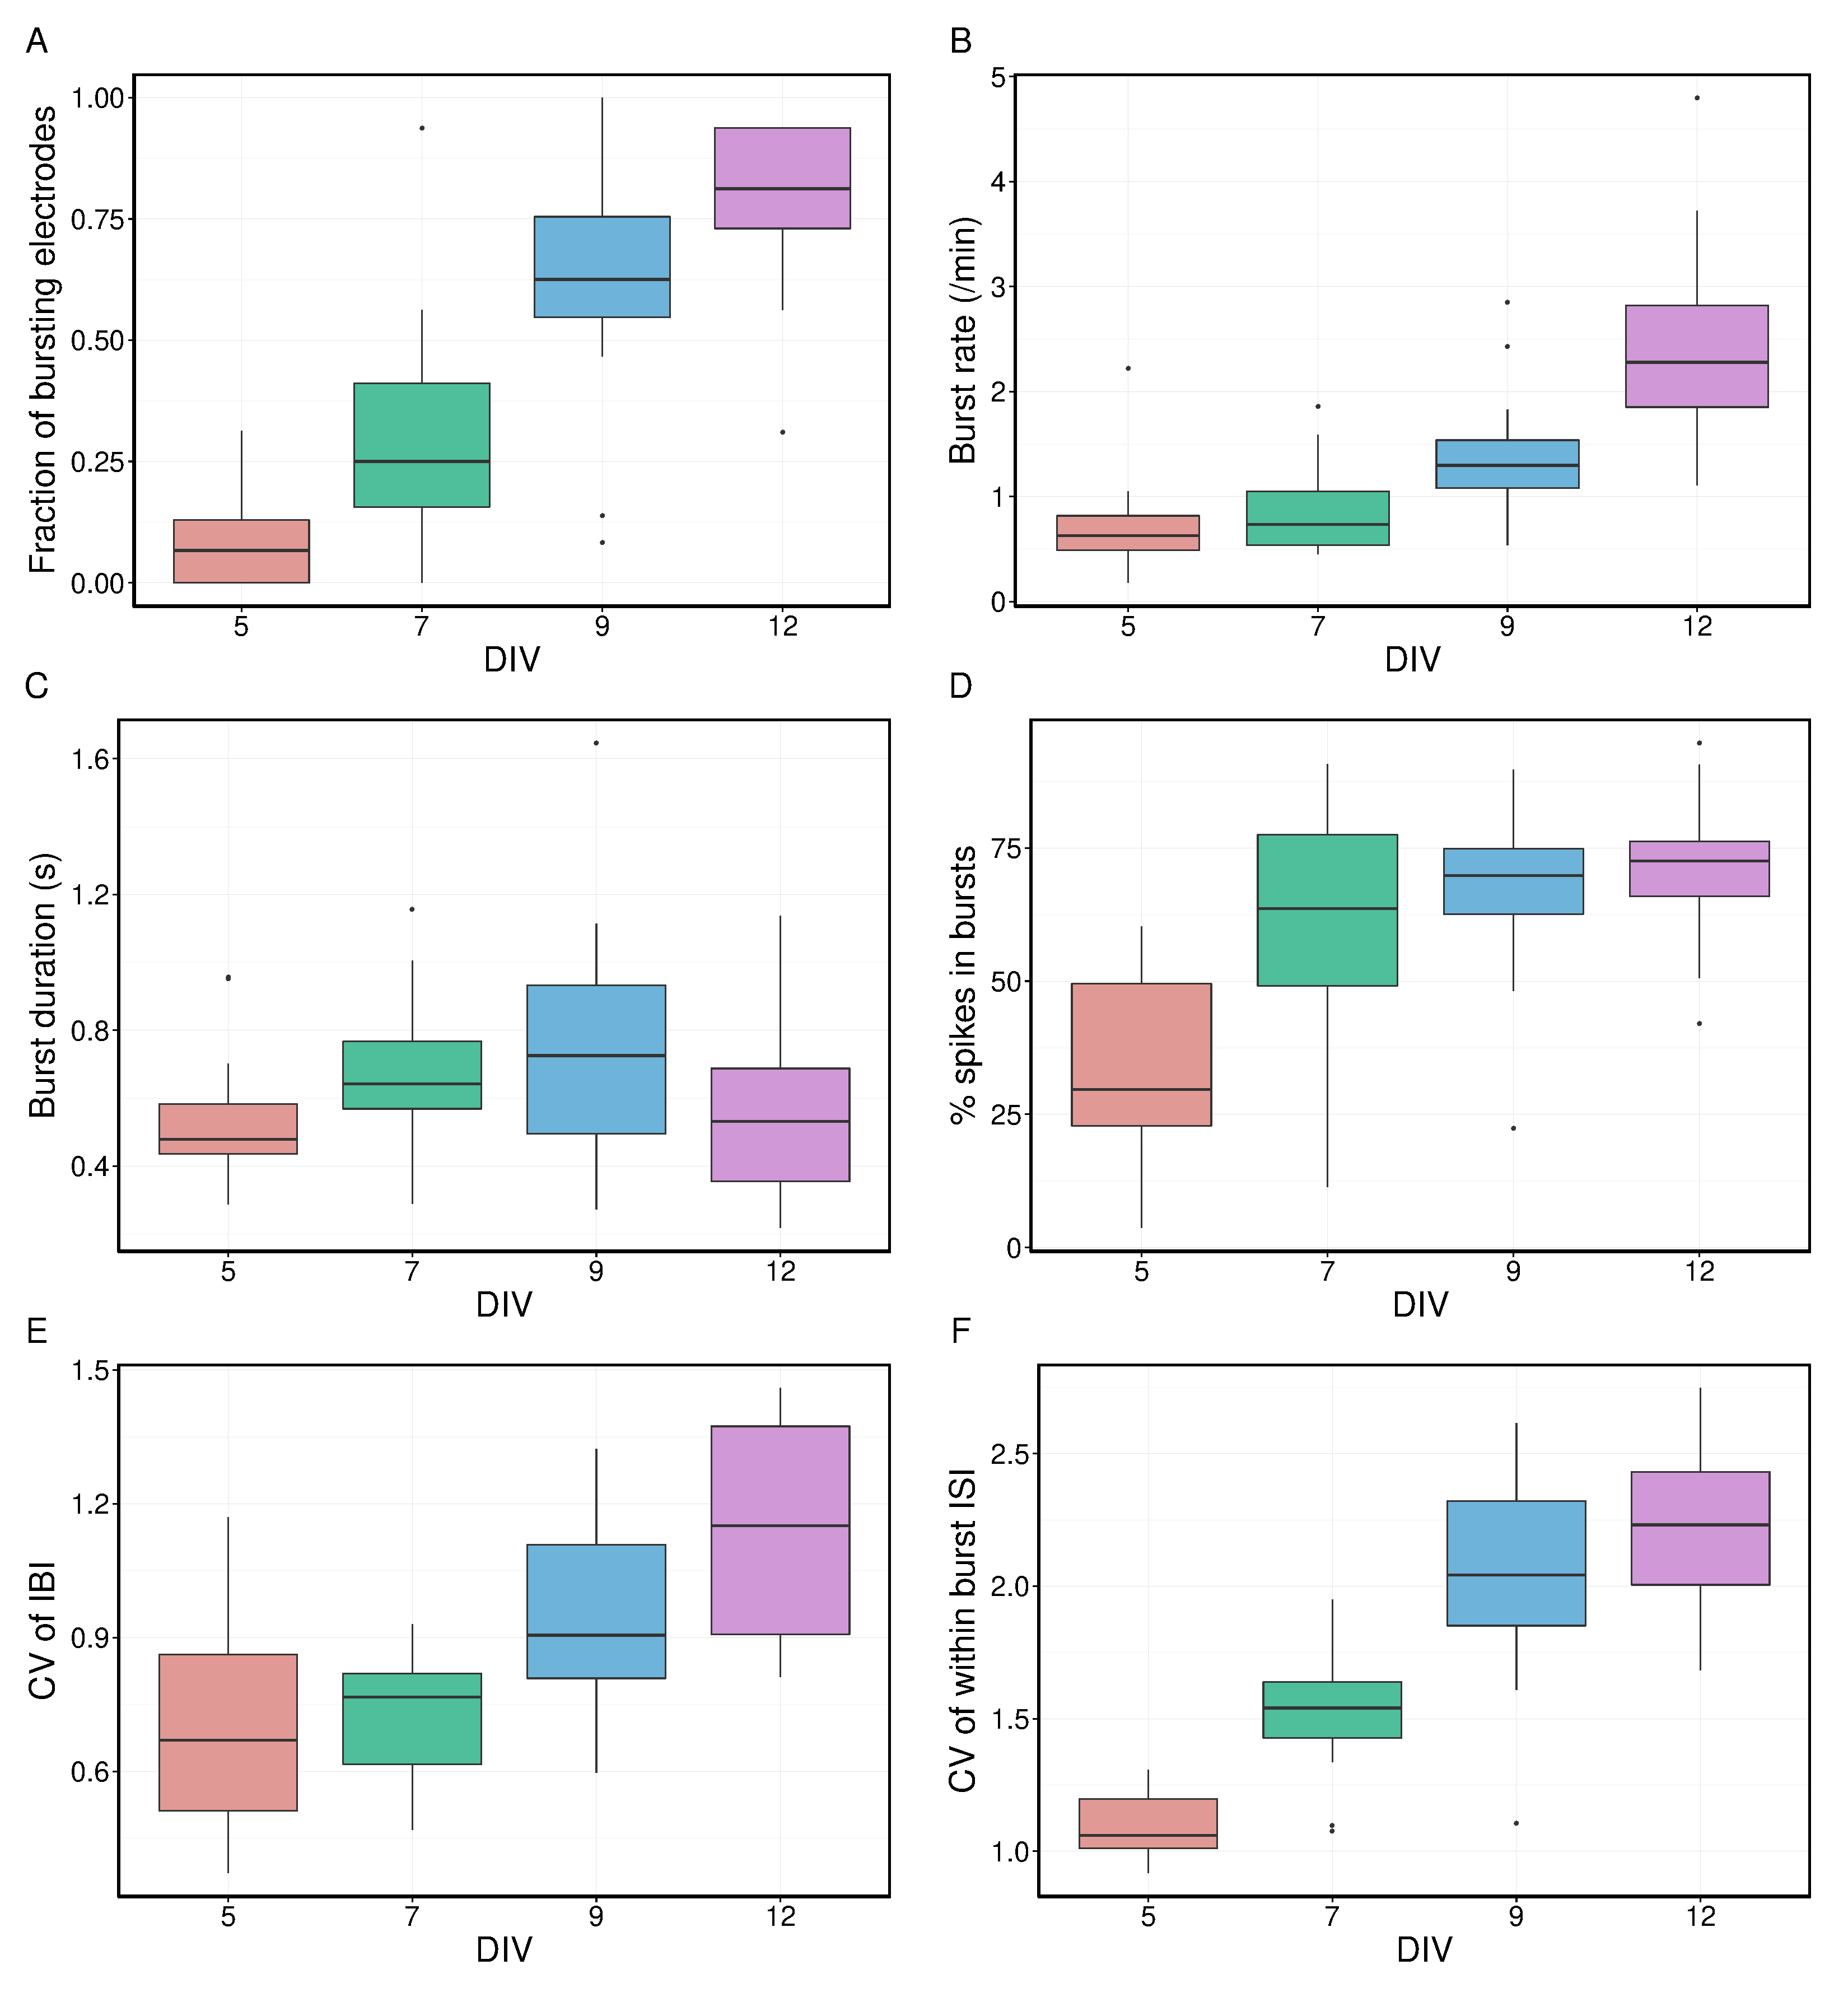
\includegraphics[width=170mm]{bursts.pdf}}
  \caption{A Fraction of bursting electrodes, B bursts per minute, C
burst duration, D percentage of spikes in bursts, E CV of IBI, and F
CV of within burst ISI.}
\end{figure}

\begin{figure}
  \centering
  \fbox{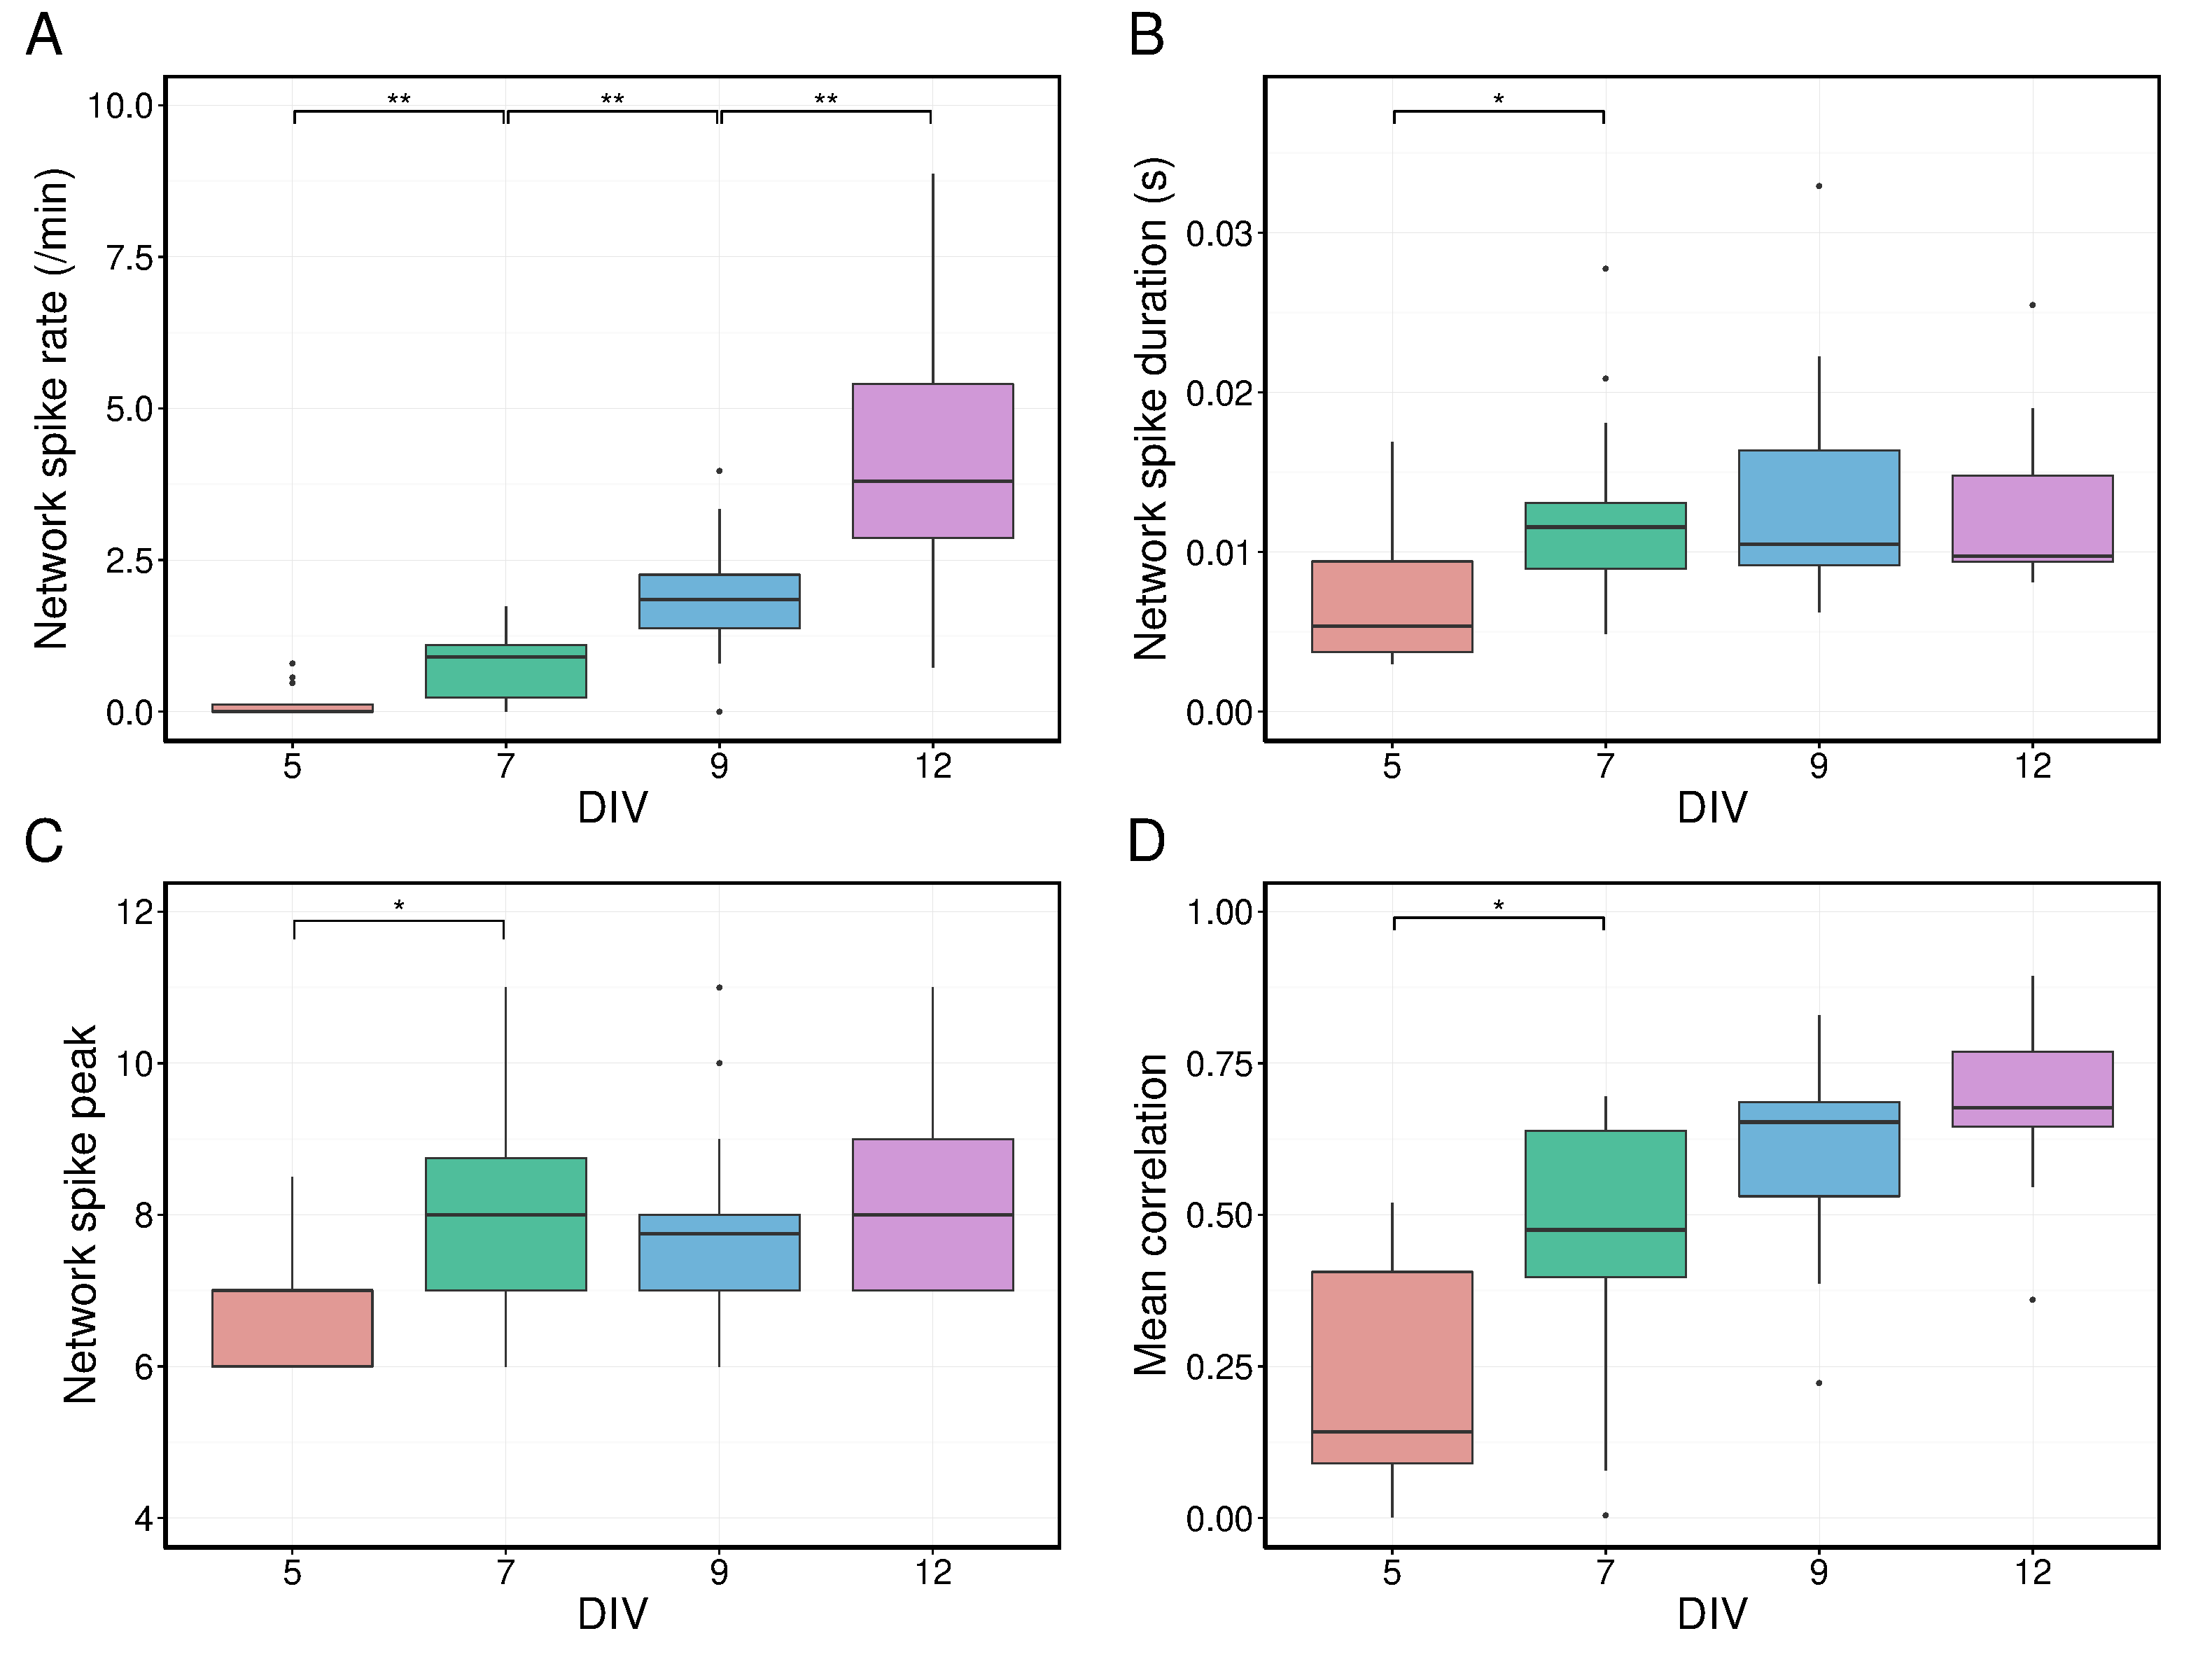
\includegraphics[width=170mm]{ns.pdf}}
  \caption{A Network spike rate, B network spike peak, C network spike
duration, and D mean correlation.}
\end{figure}

\begin{figure}
  \centering
  \fbox{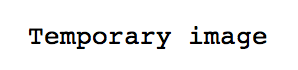
\includegraphics{temp.png}}
  \caption{[Top left] Well-level PCA projection of 12-dimensional
feature vectors onto PC dimension 1 (x-axis) and 2 (y-axis).  Each dot
represents a well, colored by day in vitro (DIV) of recording. Rough
ordering from youngest (lightest, DIV 5) to oldest (darkest, DIV 12)
wells is apparent in darkening of colors along the positive direction
. (Top right) Scree plot displays \% variance explained by the number
of PC dimensions. [Bottom left] Plate-level PCA projection of plate
averages onto PC dimension 1 (x-axis) and 2 (y-axis).  As in top,
rough ordering of observations by DIV is apparent in the light to dark
transition along the x-axis. (Bottom right) Scree plot of plate-level
PCA. Compared to the well-level PCA scree plot, a larger amount of
variation is captured in the first two PC dimensions indicating that
well averaging reduces variability.
}
\end{figure}

\begin{figure}
  \centering
   \fbox{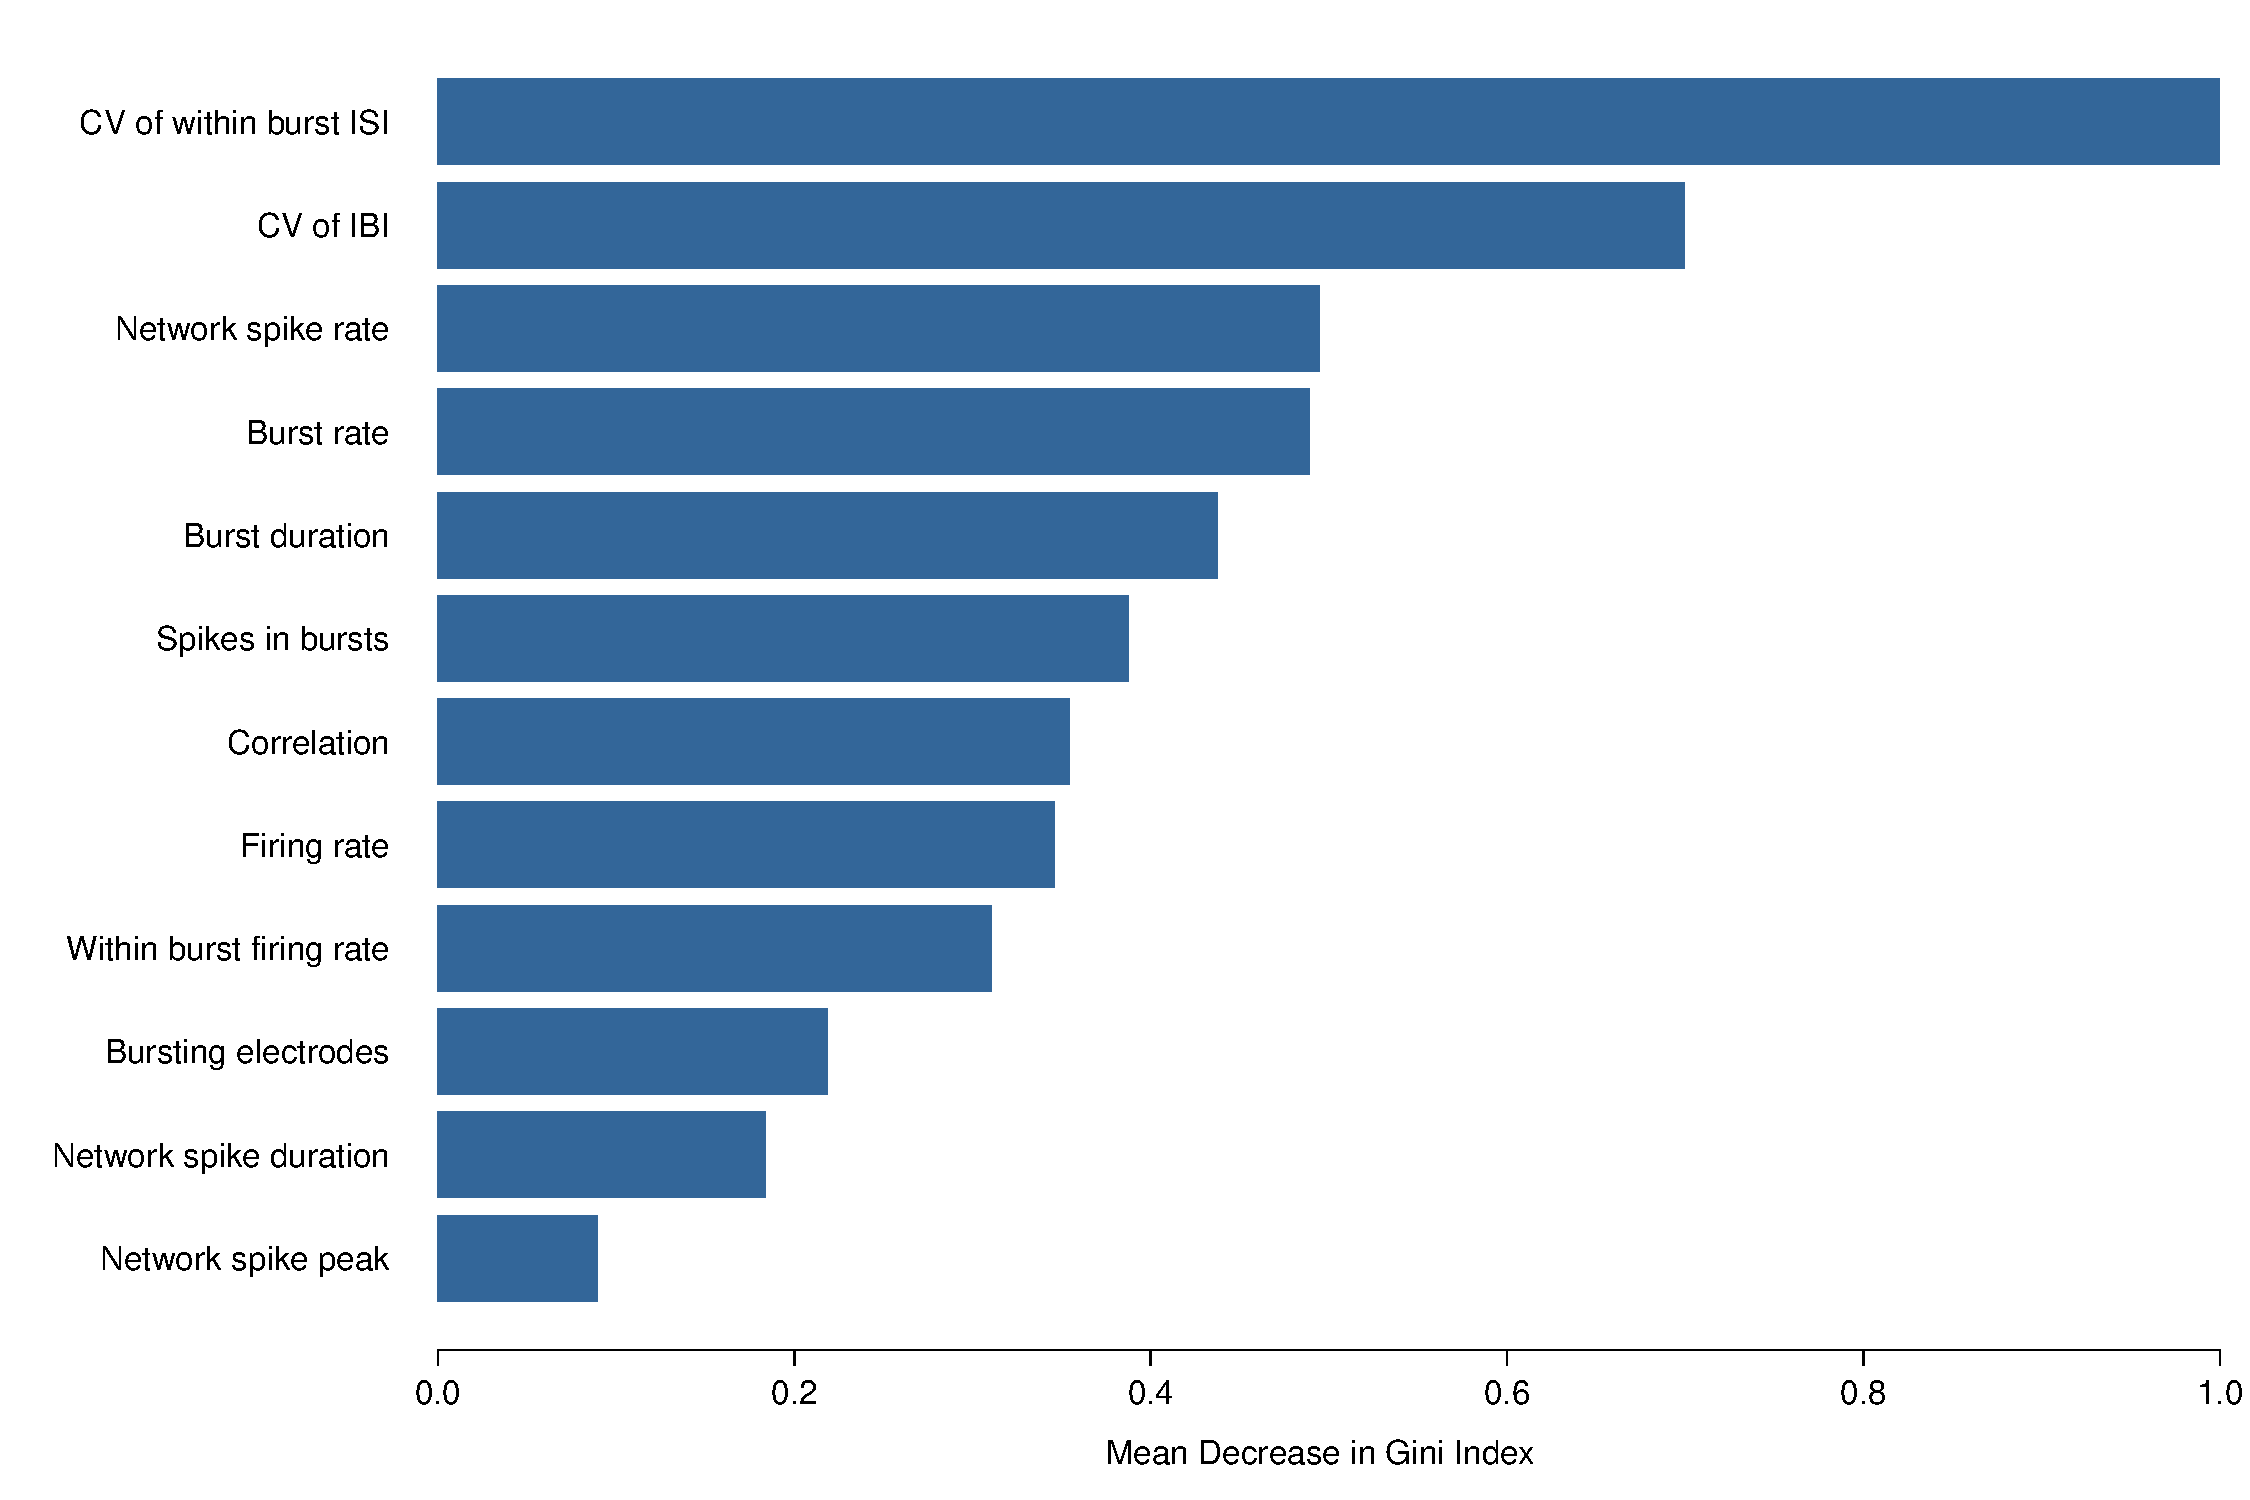
\includegraphics[width=170mm]{importance.pdf}}
  \caption{Average importance of features in driving classification,
    relative to the most important feature.}
\end{figure}

\begin{figure}
	\centering
	\fbox{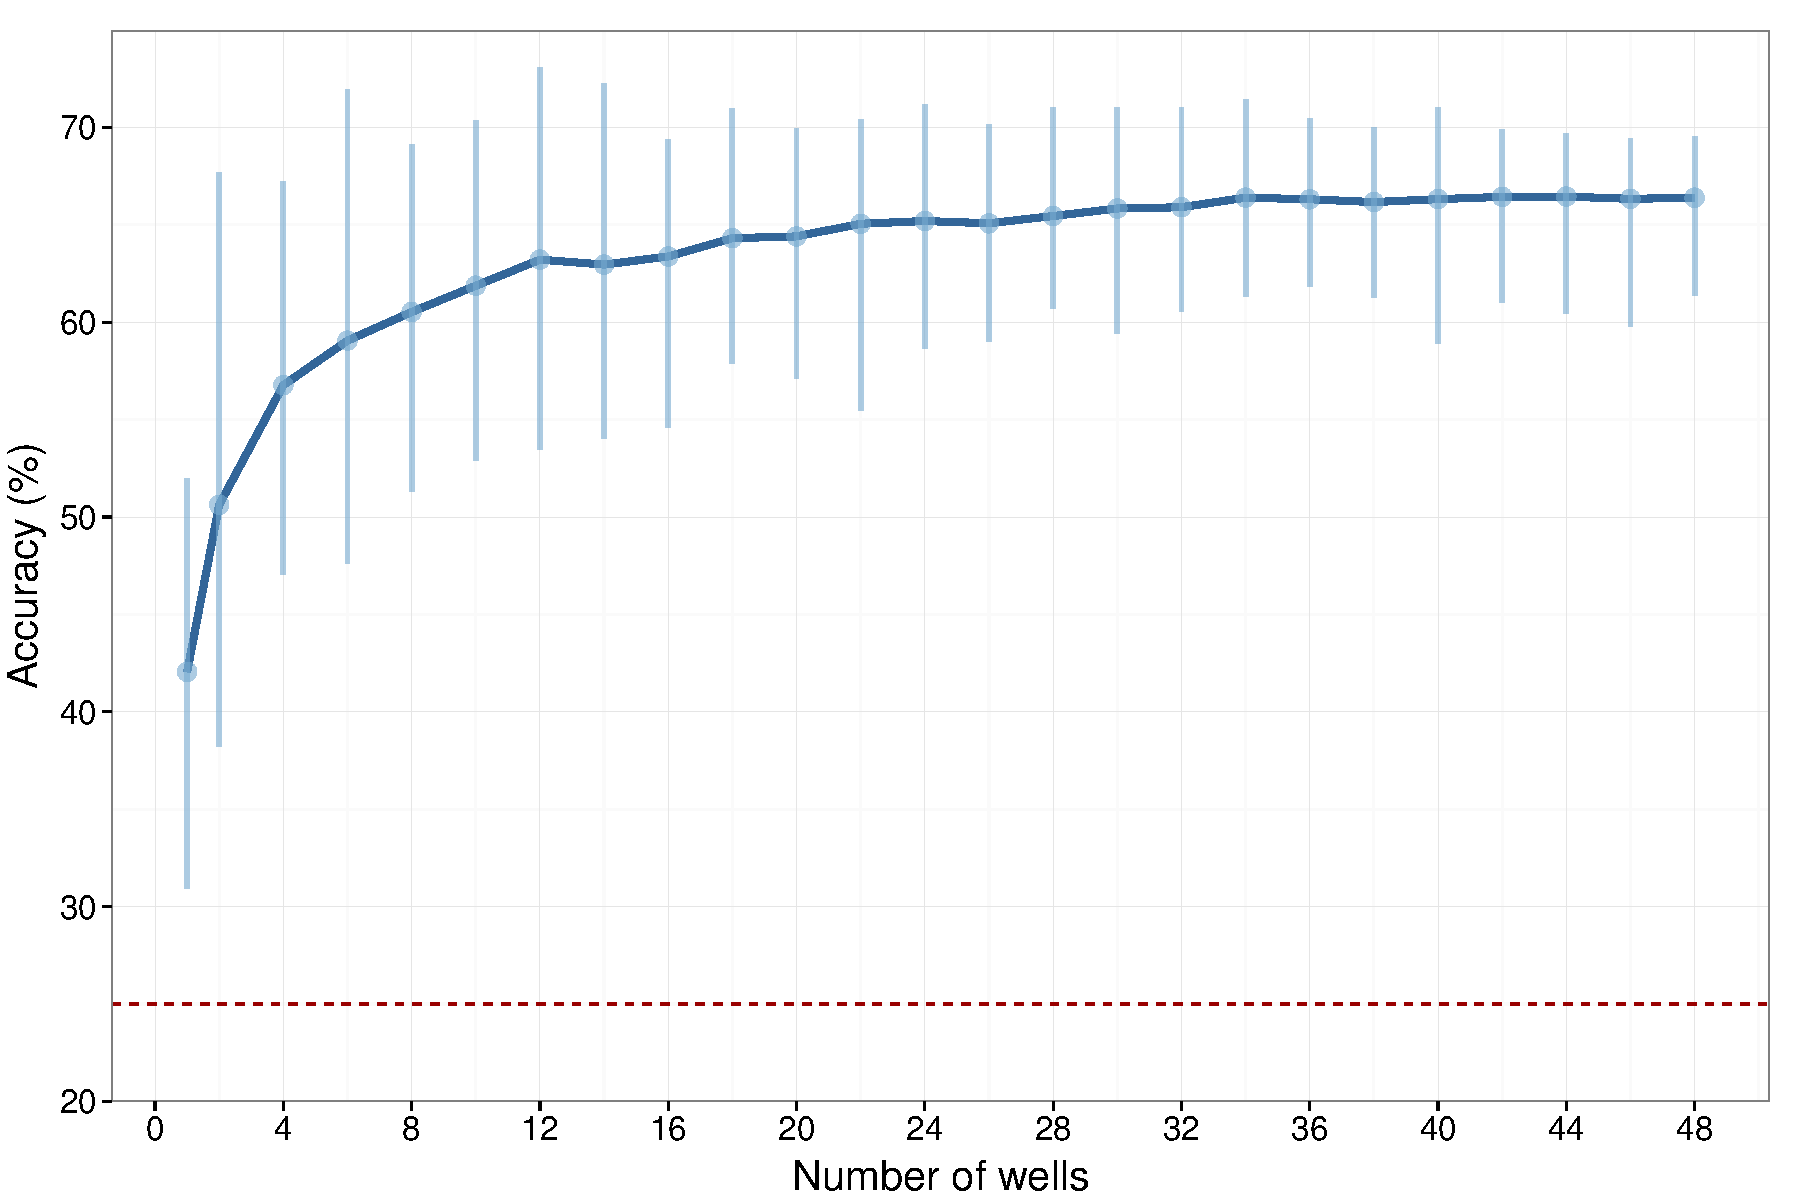
\includegraphics[width=170mm]{accuracy.pdf}}
	\caption{Accuracy of predicting the age of each plate using $n \leq 48$ wells on each plate. Dark blue line shows the mean accuracy, while the vertical lines show the minimum and maximum accuracy over 100 trials with random choices of wells.}
\end{figure}

\begin{table}
  \centering
  \rowcolors{1}{white}{gray!25}
  	\begin{tabular}{|l|m{11cm}|}
  		\hline
  		Feature & Description
  		\\ \hline 
  		Firing rate & The mean firing rate on each electrode was calculated. The well value was the median value of all active electrodes.
  		\\ Within burst firing rate & Bursts were detected using an implementation of the MaxInterval method by Neuroexplorer (Nex Technologies, 2012), with the following threshold parameters: maximum ISI $0.25\,$s, maximum beginning ISI $0.1\,$s, minimum ISI $0.8\,$s, minimum burst duration $0.05\,$s and minimum number of spikes in a burst of 6. The electrode value was the mean firing rate within all bursts on the electrode. The well value was the median  value from all electrodes that exhibited bursting behaviour.
  		\\ Fraction of bursting electrodes & An electrode was classified as bursting if the burst rate on the electrode was at least one per minute. The well value was the number of electrodes classified as bursting as a fraction of the total number of active electrodes on the well. 
  		\\ Burst rate & The number of bursts per minute on an electrode was calculated. The well value was the median value from all electrodes that exhibited bursting behaviour. 
  		\\ Burst duration  & The mean duration of all bursts on an electrode over the recording period was calculated. The well value was the median value from all electrodes that exhibited bursting behaviour. 
  		\\ Percentage of spikes in bursts & The number of spikes on an electrode classified as being within bursts divided by the total number of spikes on the electrode. The well value was the median value from all electrodes that exhibited bursting behaviour. 
  		\\ CV of IBI & The ratio of the standard deviation to the mean of the length of all interburst intervals on an electrode. The well value was the median value from all electrodes that exhibited bursting behaviour. 
  		\\ CV of within burst ISIs &  The ratio of the standard deviation to the mean of the length of all interspike intervals within bursts on an electrode. The well value was the median value from all electrodes that exhibited bursting behaviour. 
  		\\ Network spike rate & The recording period was divided into 3ms bins, and the number of electrodes on a well that fired at least one spike during each bin was counted. A network spike was defined as a period in which the number of active electrodes exceeded the threshold value of 5. The well value was the number of network spikes on the well per minute of the recording period.
  		\\ Network spike peak & The maximum number of active electrodes during each network spike. The well value was taken as the median peak value of all network spikes on the well during the recording period.
  		\\ Network spike duration & The duration of a network spike was defined as the length of time during which the  number of active electrodes on the well exceeded the threshold value. The well value was taken as the median duration of all network spikes on the well during the recording period.
  		\\ Mean correlation & The correlation between every pairwise combination of electrodes on a well was calculated using the spike time tiling coefficient (Cutts \& Eglen, 2015) with $\Delta t = 50ms$. The well value was the mean of the pairwise correlations between all distinct electrodes on the well.
  		\\ \hline
  	\end{tabular}
  \caption{Features used in our analysis and a brief description of how
    they were calculated.}
\end{table}

\begin{table}
  \centering
  \rowcolors{2}{white}{gray!25}
  \begin{tabular}{|l|c|}
  	\hline
  	\textbf{Feature removed} & \textbf{Accuracy}
  	\\ \hline 
  	CV of within burst ISI & 49.1
  	\\CV of IBI & 58.2
  	\\ Network spike rate& 62.7
  	\\ Burst rate & 65.0
  	\\ Burst duration& 66.1
  	\\ \% Spikes in bursts & 68.7
  	\\Correlation & 69.6
  	\\Firing rate & 71.3
  	\\Within burst firing rate & 72.6
  	\\Bursting electrodes & 72.8
  	\\ Network spike duration & 73.4
  	\\Network spike peak & 73.0
  	\\ \hline
  \end{tabular}
  \caption{Classifier performance at predicting the age of
arrays. Features are listed in decreasing order of importance, and the
value in each row n=1,...,12 is the mean percentage of correct
classifications using the top n features.}
\end{table}

\begin{table}
  \centering
  \rowcolors{2}{gray!25}{white}
  \begin{tabular}{|l|c|c|c|c|c|c|}
	  \hline
	  \textbf{Feature removed} & \multicolumn{5}{c}{\textbf{Accuracy}} & 
	  \\ \hline
	  & 5 vs 7 & 5 vs 9 & 5 vs 12 & 7 vs 9 & 7 vs 12 & 9 vs 12
	  \\ \hline 
		CV of within burst ISI & 75.1 & 87.4 & 88.9 & 70.1 & 78.3 & 57.2
		\\ CV of IBI & 77.4 & 89.6 & 93.8 & 77.2 & 85.3 & 65.1
		\\ Network spike rate& 79.6 & 90.4 & 95.4  & 79.6 & 88.0 & 69.1
		\\ Burst rate & 79.3 & 90.3 & 95.2 & 80.9 & 88.5 & 72.6
		\\ Burst duration& 80.2 & 90.7 & 95.3 & 81.1 & 88.7 & 73.9
		\\ \% Spikes in bursts & 81.7 & 91.1 & 95.7 & 81.6 & 90.4 & 76.7
		\\ Correlation & 82.3 & 92.1 & 95.7 & 82.3 & 91.1 & 77.2
		\\ Firing rate & 82.3 & 91.9 & 95.6 & 81.9 & 90.9 & 80.6
		\\ Within burst firing rate & 83.8 & 92.8 & 96.3 & 82.5 & 91.7 & 81.2
		\\ Bursting electrodes & 83.6 & 92.5 & 96.3 & 82.6 & 91.9 & 81.6
		\\ Network spike duration & 83.9 & 92.8 & 97.0 & 83.0 & 92.6 & 81.7
		\\ Network spike peak & 83.5 & 92.5 & 96.8 & 82.9 & 92.9 & 82.1
	\\ \hline
\end{tabular}
  \caption{Classifier performance at predicting the age of arrays for
    each pairwise combination of DIV. Features are listed in
    decreasing order of importance, and the value in each row
    n=1,...,12 is the mean percentage of correct classifications using
    the top n features.}
\end{table}



\end{document}
